\documentclass{article}

\usepackage[french]{babel}
\usepackage[utf8]{inputenc}
\usepackage{graphicx}
\usepackage{subcaption}

%%%%%%%%%%%%%%%% Lengths %%%%%%%%%%%%%%%%
\setlength{\textwidth}{15.5cm}
\setlength{\evensidemargin}{0.5cm}
\setlength{\oddsidemargin}{0.5cm}

%%%%%%%%%%%%%%%% Variables %%%%%%%%%%%%%%%%
\def\projet{0}
\def\titre{Résolution de systèmes linéaires / Application à l'équation de la chaleur}
\def\groupe{4}
\def\equipe{4}
\def\responsible{acattarin}
\def\secretary{electakone}
\def\others{mchellaf, bchenard}

\begin{document}

%%%%%%%%%%%%%%%% Header %%%%%%%%%%%%%%%%
\noindent\begin{minipage}{0.98\textwidth}
  \vskip 0mm
  \noindent
  { \begin{tabular}{p{7.5cm}}
      {\bfseries \sffamily
        Projet \projet} \\ 
      {\itshape \titre}
    \end{tabular}}
  \hfill 
  \fbox{\begin{tabular}{l}
      {~\hfill \bfseries \sffamily Groupe \groupe\ - Equipe \equipe
        \hfill~} \\[2mm] 
      Responsable : \responsible \\
      Secrétaire : \secretary \\
      Codeurs : \others
    \end{tabular}}
  \vskip 4mm ~

  ~~~\parbox{0.95\textwidth}{\small \textit{Résumé~:} \sffamily  }
  \vskip 1mm ~
\end{minipage}

%%%%%%%%%%%%%%%% Main part %%%%%%%%%%%%%%%%
\section{Décomposition de Cholesky}
\label{sec:decomp_cholesky}

\subsection{Factorisation complète}
\label{ssec:factor_compl}
L'algorithme de la factorisation dense de Cholesky peut s'écrire ainsi:
\begin{verbatim}

fonction cholesky(A : matrice symétrique définie positive) -> T : matrice triangulaire inférieure
    n = taille(A)
    T = matrice de zéros de taille n x n
    pour i allant de 0 à n-1 faire
        pour j allant de 0 à i-1 faire
            somme = 0
            pour k allant de 0 à j-1 faire
                somme = somme + T[i,k] * T[j,k]
            fin pour
            T[i,j] = (A[i,j] - somme) / T[j,j]
        fin pour
        somme = 0
        pour k allant de 0 à i-1 faire
            somme = somme + T[i,k]^2
        fin pour
        T[i,i] = racine_carree(A[i,i] - somme)
    fin pour
    retourner T
fin fonction

\end{verbatim}

Cet algorithme a une complexité en O($n^3$) avec n la taille de la matrice A prise en paramètre.

Pour résoudre un système linéaire du type A.x=b en utilisant la factorisation de Cholesky, il y a plusieurs étapes : 
\begin{itemize}
    \item La décomposition de Cholesky : on doit calculer la matrice triangulaire inférieure T telle que A=$TT^{T}$. Cela peut être fait en utilisant l'algorithme de décomposition de Cholesky décrit précédemment.
    \item La résolution du système triangulaire : on doit résoudre deux systèmes linéaires triangulaires, l'un inférieur T.y=b et l'autre supérieur $T^{T}$x=y. Ces systèmes linéaires triangulaires peuvent être résolus en temps linéaire, car les matrices sont triangulaires. 
\end{itemize}
La complexité de la résolution d'un système triangulaire est en O($n^2$). Ainsi, la complexité totale de la résolution d'un système linéaire dense est: O($n^3$ + $n^2$) soit O($n^3$). 

\subsection{Factorisation incomplète}
\label{ssec:factor_incompl}
La factorisation de Cholesky incomplète suit la factorisation complète à l'exception que lorsque A[i][j] = 0 , on mettra T[i][j] à 0. Ceci évite de faire des calculs inutiles. 
Il faut d'abord écrire un algorithme pour générer des matrices symétriques définies positives creuses avec un nombre de termes extra-diagonaux non nuls réglable. Pour cela, il y a plusieurs étapes:
\begin{itemize}
    \item On génère une matrice carrée de taille n avec des termes aléatoires.
    \item On met $n^2$ - k termes à 0 (k est le nombre de termes extra-diagonaux non nuls réglable).
    \item On rend la matrice symétrique en effectuant l'opération : A = 0.5.(A+$A^{T}$)
    \item On rend la matrice définie postive en calculant : A = A.$A^{T}$.

\end{itemize}

Pour tester la factorisation incomplète, il faut d'abord tester si la matrice générée par notre algorithme est bien creuse symétrique et définie positive puis ensuite vérifier si la matrice obtenue après factorisation est bien correcte. 
Pour cela, on peut utiliser la fonction \verb|numpy.linalg.cholesky()|. Cette fonction renvoie une erreur si la matrice en entrée n'est pas définie postive et la matrice T théorique que l'on doit obtenir avec notre algorithme.

La complexité de la factorisation de Cholesky incomplète ne dépend plus de la taille de la matrice comme pour la factorisation complète mais du nombre de termes non nuls. En effet, puisque l'on effectue des calculs que lorsque l'on a A[i][j] $\ne$ 0.
Ainsi, si l'on a k le nombre de termes nuls, la complexité est : O($k^2$). Lgit a complexité est donc bien meilleure que celle de la factorisation de Cholesky complète.

Le conditionnement d'une matrice est une mesure de la sensibilité de la solution d'un système linéaire par rapport aux perturbations des données d'entrée. Un conditionnement élevé indique que des petites perturbations dans les données d'entrée peuvent provoquer des variations importantes dans la solution du système linéaire.
Ainsi, ici, on considère que lorsque que le conditionnement est inférieur au préconditionnement, alors il est de bonne qualité.
Pour étudier le conditionnement des matrices obtenues avec les factorisations de Cholesky complète et incomplète., on utilisera les fonctions \verb|np.linalg.cond| et \verb|np.inv()|.
Puisque la factorisation incomplète effectue moins d'opérations, on obtient de meilleurs conditionnements avec cette méthode plutôt qu'avec la factorisation de Cholesky complète.

En résumé, cette partie a exploré les différents aspects de la factorisation de Cholesky et de la factorisation de Cholesky incomplète, en mettant l'accent sur leur efficacité pour les matrices creuses. 
Nous avons également examiné la qualité des préconditionneurs obtenus à partir de ces méthodes et avons conclu que la factorisation de Cholesky incomplète donne de meilleurs résultats.
\section{Méthode du gradient conjugué}
\label{sec:meth_grad_conj}

\section{Application à l'équation de la chaleur}
\label{sec:eq_chaleur}

\subsection{Fonctions principales}
\label{ssec:fonc_princ}
Grâce à la discrétisation numérique, l'équation de la chaleur peut être ramenée à la résolution d'un système linéaire. 
La matrice représentant l'opérateur Laplacien étant donnéé, il a suffit de créer la fonction permettant de la construire.
Cette fonction possède une compléxité en $\Theta(N²)$, étant donné qu'on parcours toute la matrice.

Ensuite, nous avons mis en place des "situations" où certains points étaient sources de chaleur. Cela à permis de voir comment se comportait l'algorithme dans des cas de figures différents. Nous représenterons ici que quelques cas, les autres peuvent être observés à l'exécution du programme python \emph{chaleur.py}. Ces simulations (disponibles nous ont permis d'observer facilement les résultats aberrant et donc de détecter de potentiels problèmes dans nos algorithmes.



\subsection{Fonctions auxiliaires}
\label{ssec:fonc_aux}
Il a été nécessaire de mettre en place des fonctions permettant de passer un vecteur en matrice et inversement.
En effet, pour pouvoir afficher les \emph{Heat maps} il a fallu utiliser des matrices. Cependant, afin de résoudre l'équation linéaire, l'environnement de taille $N$*$N$ est représenté comme étant un vecteur de taille $N²$.

Il a aussi fallu mettre en place une fonction permettant donc d'afficher les \emph{Heat maps}. Pour cela nous avons utilisé matplotlib.
Le module possédant déjà une option pour afficher des gradients de température, il nous a juste fallu s'approprier le code.


\subsection{Résultats}
\label{ssec:res}
Ci-dessous se trouvent nos résultats pour deux situations : la première possédant une source de chaleur centrale, la seconde avec un mur de chaleur sur un côté supérieur.

\begin{figure}[ht]
  \centering
  \begin{subfigure}{0.3\textwidth}
    \centering
    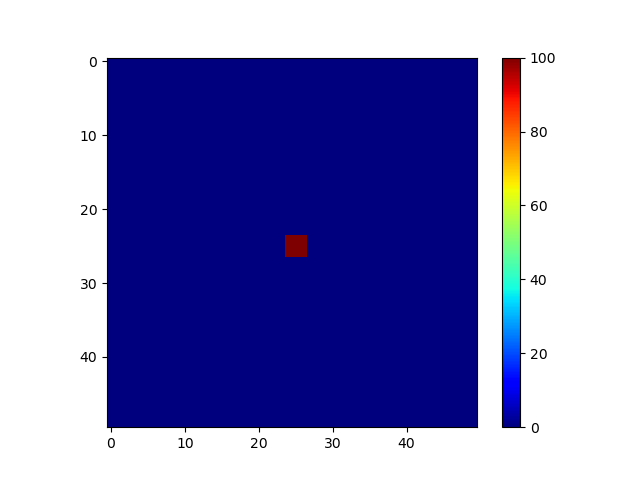
\includegraphics[width=\linewidth]{Chaleur_1.png}
    \caption{Carte de la source de chaleur}
    \label{subfig:central_source_prev}
  \end{subfigure}
  \hfill
  \begin{subfigure}{0.3\textwidth}
    \centering
    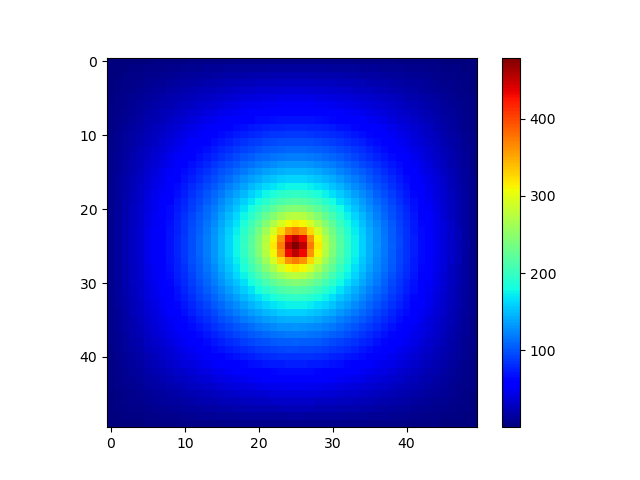
\includegraphics[width=\linewidth]{Chaleur_1b.png}
    \caption{Carte de la répartition de la température}
    \label{subfig:central_source_temp}
  \end{subfigure}
  \hfill
  \begin{subfigure}{0.3\textwidth}
    \centering
    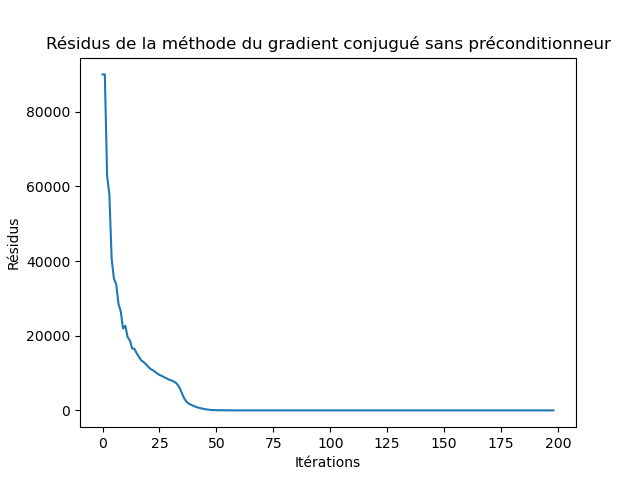
\includegraphics[width=\linewidth]{Chaleur_1c.png}
    \caption{Evolution du résidu de la méthode du gradient conjugué}
    \label{subfig:central_source_residus}
  \end{subfigure}
  \caption{Simulation du cas d'une source de chaleur centrale}
  \label{fig:central_source}
\end{figure}

\begin{figure}[ht]
  \centering
  \begin{subfigure}{0.3\textwidth}
    \centering
    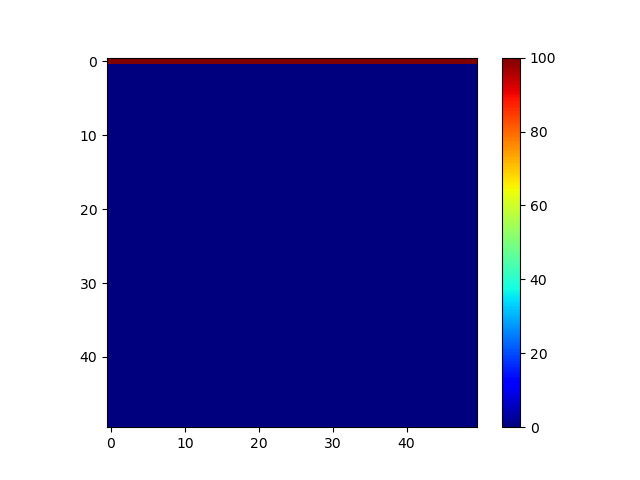
\includegraphics[width=\linewidth]{Chaleur_2.png}
    \caption{Carte de la source de chaleur}
    \label{subfig:heat_wall_prev}
  \end{subfigure}
  \hfill
  \begin{subfigure}{0.3\textwidth}
    \centering
    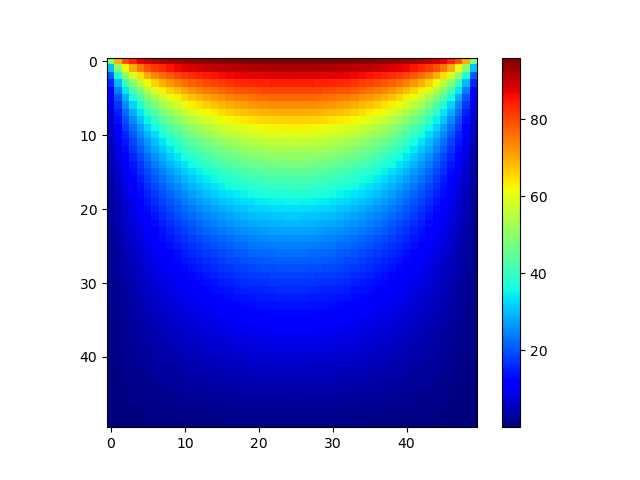
\includegraphics[width=\linewidth]{Chaleur_2b.png}
    \caption{Carte de la répartition de la température}
    \label{subfig:heat_wall_temp}
  \end{subfigure}
  \hfill
  \begin{subfigure}{0.3\textwidth}
    \centering
    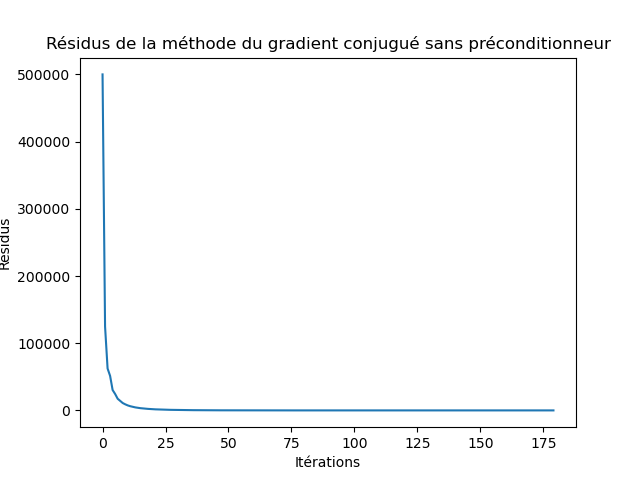
\includegraphics[width=\linewidth]{Chaleur_2c.png}
    \caption{Evolution du résidu de la méthode du gradient conjugué}
    \label{subfig:heat_wall_residus}
  \end{subfigure}
  \caption{Simulation du cas d'un mur de chaleur}
  \label{fig:heat_wall}
\end{figure}

Nos algorithmes semblent fonctionner puisque nous ne remarquons pas d'aberrations dans ces illustrations. Ces méthodes constituent donc une bonne approximation de la solution de l'équation de la chaleur, d'autant plus que les programmes se terminent toujous avec un résidus très proche de 0.

\end{document}
